%%%%%%%%%%%%%%%%%%%%%%%%%%%%%%%%%%%%%%%%%
% Report Template
% LaTeX Template
% Version 1.2 (2023-06-29)
%
% This template was adapted by:
% Jonathan Decker (jonathan.decker@uni-goettingen.de)
% Adapted from the informatics master and bachelor thesis template
% offered by the University Göttingen
% https://www.uni-goettingen.de/de/626775.html
%
%%%%%%%%%%%%%%%%%%%%%%%%%%%%%%%%%%%%%%%%%
\documentclass[12pt, a4paper, hidelinks]{article}
\usepackage{graphicx}
\usepackage{hyperref}
\usepackage{xcolor}
\usepackage{url}
\usepackage[english]{babel}
\usepackage[nottoc]{tocbibind}
\usepackage[utf8]{inputenc}
\usepackage[T1]{fontenc}
\usepackage[backend=biber,style=alphabetic]{biblatex}
\addbibresource{ref.bib} % The filename of the bibliography
\usepackage[left=2.5cm,right=2.5cm,top=2.5cm,bottom=2.5cm]{geometry}
\usepackage{acronym}
\usepackage{fancyhdr}
\pagestyle{fancy}
\usepackage{lipsum}
\usepackage{array, tabularx, booktabs} % For better tables
\usepackage{longtable}
\usepackage{minted}
\usemintedstyle{tango}
\setminted{linenos, autogobble, bgcolor=gray!5}
\usepackage{titlesec}
\usepackage{amssymb}
\setlength{\marginparwidth}{2cm}
\usepackage{todonotes}
\usepackage{nicematrix}
\usepackage[autostyle=true]{csquotes}
\usepackage{cleveref}
\usepackage{listings}


% \usepackage[english]{babel}
% \usepackage{natbib}

\titleformat{\section}[hang]{\huge\bfseries}{\thesection\hspace{20pt}}{0pt}{\huge\bfseries}
\graphicspath{{figures/}{./}{assets/}}

\newcommand{\ccheckmark}{\mbox{\ooalign{$\checkmark$\cr\hidewidth$\square$\hidewidth\cr}}}
\newcommand{\ccheckbox}{\mbox{$\square$}}

% --- document configuration ---

\newcommand{\thesistitle}{Smart Injection of Environment Variables in Kubernetes Pod}
\newcommand{\supervisor}{Jonathan Decker}
\newcommand{\authorname}{Pranay Bhatia}
\newcommand{\university}{Georg-August-Universität Göttingen}
\newcommand{\department}{Institute of Computer Science}
\newcommand{\thesistype}{Seminar Report}
\newcommand{\matrikelnumber}{17935037}
\newcommand{\keywords}{} % Set keywords that describe your report

\hypersetup{pdftitle=\thesistitle} % Set the PDF's title to your title
\hypersetup{pdfauthor=\authorname} % Set the PDF's author to your name
\hypersetup{pdfkeywords=\keywords} % Set the PDF's keywords to your keywords

\begin{document}

\fancyhead{}
\fancyhead[R]{\footnotesize \thesistitle}
\fancyfoot{}
\fancyfoot[R]{\thepage}
\fancyfoot[L]{Section \thesection}
\fancyfoot[C]{\authorname}
\renewcommand{\headrulewidth}{0.4pt}
\renewcommand{\footrulewidth}{0.4pt}

\pagestyle{plain}
% --- title page ---

\begin{titlepage}
\begin{minipage}[t]{0.6\textwidth}
\begin{flushleft}

\includegraphics[width=6.5cm]{logo-goettingen.pdf}
\end{flushleft}
\end{minipage}
\begin{minipage}[t]{0.4\textwidth}
\begin{center}
\qquad
\includegraphics[width=2.5cm]{hps-logo.pdf}
\end{center}
\end{minipage}

\begin{center}

\vspace*{.06\textheight}
\LARGE \thesistype\\[0.5cm]

\rule{.9\linewidth}{.6pt} \\[0.4cm] % Horizontal line
{\huge \bfseries \thesistitle}\vspace{0.4cm}
\rule{.9\linewidth}{.6pt} \\[1.5cm] % Horizontal line

\Large\authorname\\
\hfill\\
\large MatrNr: \matrikelnumber\\ \vfill
Supervisor: \supervisor
\vfill
\university\\
\department
\vfill
{\large \today}\\[4cm] % Date

\vfill
\end{center}
\end{titlepage}

% --- abstract ---

\newpage
\pagenumbering{roman}
\setcounter{page}{1}

\section*{Abstract}
\textbf{Automating Kubernetes Pod Restarts with Dynamic Environment Variable Injection using HashiCorp Vault}

\medskip

In the realm of Kubernetes orchestration, automating the dynamic injection of environment variables into running pods has been a longstanding challenge. This research introduces a novel solution that leverages HashiCorp Vault and a Kubernetes liveness probe to facilitate automated restarts of pods upon changes to environment variables.

Traditional solutions for injecting secrets into pods at startup lack the capability to handle dynamic updates without manual intervention. This research addresses the difficulty of achieving automated restarts when environment variables within a pod need to be modified, presenting a comprehensive solution for seamless integration.

Current industry-standard solutions, such as HashiCorp Vault, excel at secret injection during pod initialization. However, they fall short in automating pod restarts when environment variables change, requiring manual restarts or reliance on DevOps processes. This limitation hinders the efficiency and agility of managing dynamic configurations.

Our innovative approach introduces a liveness probe within Kubernetes, ensuring constant monitoring of the environment variable path within the pod. If changes are detected, the liveness probe communicates with HashiCorp Vault, retrieves the updated variables, and triggers a controlled restart of the main container. This self-contained solution eliminates the need for manual interventions and provides a seamless mechanism for automated updates.

The proposed solution has been successfully implemented, demonstrating its effectiveness in automating pod restarts upon changes to environment variables. The evaluation revealed that the solution operates with minimal overhead, ensuring a reliable and efficient mechanism for maintaining up-to-date configurations within a dynamic Kubernetes environment.

In summary, this research introduces an automated solution to a prevalent challenge in Kubernetes orchestration, offering a streamlined process for dynamically updating environment variables and triggering pod restarts. The outcome demonstrates the potential for increased efficiency and autonomy in managing containerized applications, paving the way for more responsive and adaptive Kubernetes deployments.





\newpage

% --- table of contents ---
% Comment out the lists you are not using
\clearpage
\phantomsection\pdfbookmark{\contentsname}{toc}
\tableofcontents
\newpage

% --- content ---

\pagenumbering{arabic}
\setcounter{page}{1}
\pagestyle{fancy}

\section{Introduction}

In modern containerized environments orchestrated by Kubernetes, managing environment variables efficiently and securely is essential for ensuring the reliability and security of applications. Environment variables play a crucial role in configuring and customizing containerized applications, providing a flexible and dynamic way to pass configuration information to running containers. However, manually updating environment variables in Kubernetes deployments can be cumbersome and error-prone, particularly in dynamic environments where configuration changes are frequent.

The aim of this report is to propose a novel approach for smartly injecting environment variables into Kubernetes clusters and automating the process of detecting changes and restarting pods accordingly. By leveraging Kubernetes' liveness probe mechanism—a built-in feature for determining the health of containerized applications—we can create a robust and automated solution for managing environment variables seamlessly.

Our approach involves encapsulating the logic for retrieving, validating, and updating environment variables within a liveness probe script, which is embedded within the container's configuration. This script continuously monitors the availability and integrity of environment variables, fetching them from a secure and centralized source, such as HashiCorp Vault. Upon detecting changes or discrepancies in the environment variables, the liveness probe triggers a pod restart, ensuring that the application remains up-to-date with the latest configuration changes.

By automating the injection and updating of environment variables in Kubernetes deployments, our approach offers several benefits, including:

\begin{itemize}
    \item Improved Reliability: Ensuring that applications always have access to the correct and up-to-date environment variables enhances the reliability and stability of Kubernetes deployments.
    
    \item Enhanced Security: By fetching environment variables from a centralized and secure source, such as HashiCorp Vault, we can enforce access controls, encryption, and audit trails, thereby enhancing the security posture of the application.
    
    \item Efficient Configuration Management: Automating the process of injecting and updating environment variables simplifies configuration management tasks, reducing the risk of human error and streamlining the deployment process.
    
    \item Dynamic Scalability: With automated environment variable injection and pod restarts, Kubernetes deployments can dynamically scale in response to changing workload demands while ensuring consistent and reliable configuration across all instances.
\end{itemize}

In this report, we present the methodology, implementation details, experimental results, and discussion of our approach for smartly injecting environment variables in Kubernetes clusters. Through empirical evaluation and analysis, we demonstrate the effectiveness and efficiency of our solution in improving the reliability, security, and manageability of Kubernetes deployments.



\section{Problem Statement}

In Kubernetes deployments, managing environment variables effectively while ensuring their timely and accurate injection into running pods poses a significant challenge. Manually updating environment variables can lead to errors, inconsistencies, and downtime, particularly in dynamic environments where configuration changes are frequent. The problem statement revolves around the need for a robust and automated solution to intelligently inject environment variables into Kubernetes clusters and automatically trigger pod restarts upon detecting changes or updates to the configuration.

\bigskip

\textbf{Key challenges include:}

\begin{enumerate}
    \item \textbf{Manual Configuration Management:} Manually updating environment variables in Kubernetes deployments is time-consuming, error-prone, and can result in configuration drifts and inconsistencies across pods.
    
    \item \textbf{Dynamic Environment:} In dynamic Kubernetes environments where pods scale up, scale down, or migrate across nodes, ensuring that all pods have access to the latest environment variables becomes challenging.
    
    \item \textbf{Security and Compliance:} Ensuring the security and confidentiality of environment variables while maintaining compliance with regulatory requirements, such as GDPR and HIPAA, is critical for protecting sensitive information.
    
    \item \textbf{Application Reliability:} Changes to environment variables, such as API keys or database credentials, may require pod restarts to take effect, impacting application availability and reliability if not handled efficiently.
    
    \item \textbf{Scalability:} As Kubernetes deployments scale to accommodate varying workloads, the process of injecting and updating environment variables must scale accordingly to meet the demands of dynamic environments.
\end{enumerate}

Addressing these challenges requires the development of an automated solution that integrates seamlessly with Kubernetes deployments, intelligently manages environment variables, and ensures the reliability, security, and scalability of applications running in Kubernetes clusters.

\section{Background and Motivation}

\subsection{HashiCorp Vault}

\textbf{Introduction:}
HashiCorp Vault is a popular open-source tool for managing secrets and sensitive data in modern cloud-native environments. It provides a centralized platform for securely storing, accessing, and managing secrets such as API keys, passwords, certificates, and encryption keys. Vault offers a robust set of features and capabilities designed to address the challenges of secrets management in dynamic and distributed systems.

\textbf{Use and Benefits:}
The primary use of HashiCorp Vault is to securely manage secrets and sensitive data in cloud-native applications and infrastructure. By centralizing the storage of secrets, Vault helps organizations improve security, compliance, and operational efficiency. Some key benefits of using HashiCorp Vault include:

\begin{itemize}
    \item \textbf{Enhanced Security:} Vault provides encryption, access control, and auditing capabilities to protect sensitive data from unauthorized access and breaches.
    
    \item \textbf{Scalability:} Vault is designed to scale horizontally to meet the needs of large and dynamic environments, ensuring that secrets management remains efficient and reliable as deployments grow.
    
    \item \textbf{Compliance:} Vault helps organizations meet regulatory compliance requirements by enforcing security best practices and providing audit trails for secret access and management.
    
    \item \textbf{Integration:} Vault seamlessly integrates with popular cloud platforms, container orchestration systems (such as Kubernetes), and CI/CD pipelines, making it easy to incorporate secrets management into existing workflows.
\end{itemize}

\textbf{Thanks to Built-in APIs:}
One of the key features of HashiCorp Vault is its rich set of built-in APIs, which allow developers and operators to interact with Vault programmatically. These APIs provide access to Vault's functionality, including the ability to retrieve, create, update, and delete secrets. Additionally, Vault offers APIs for dynamic secrets generation, token management, and encryption operations. This flexibility enables developers to automate secrets management tasks and integrate Vault seamlessly into their applications and infrastructure.

\textbf{Available APIs to Fetch Secrets:}
Vault exposes several APIs for fetching secrets, each designed to accommodate different use cases and access patterns:

\begin{itemize}
    \item \textbf{Key/Value Secrets Engine API:} This API allows users to store and retrieve secrets as key/value pairs within Vault's hierarchical data store.
    
    \item \textbf{Database Secrets Engine API:} Vault provides APIs for dynamically generating and managing database credentials, allowing applications to securely access databases without exposing static credentials.
    
    \item \textbf{AWS Secrets Engine API:} With this API, Vault can dynamically generate AWS IAM credentials with configurable TTLs and IAM policies, enabling secure access to AWS resources.
    
    \item \textbf{Kubernetes Secrets Engine API:} Vault integrates seamlessly with Kubernetes clusters, allowing applications running in Kubernetes to authenticate with Vault and fetch secrets securely using Kubernetes service accounts.
\end{itemize}

\textbf{In summary,} HashiCorp Vault is a powerful tool for managing secrets and sensitive data in cloud-native environments. Its rich set of features, flexible APIs, and seamless integrations make it an essential component of modern infrastructure and application security architectures.

\subsection{Liveness Probes}

\textbf{Functionality of Liveness Probe}

\textbf{What is Liveness Probe:}
In Kubernetes, a liveness probe is a mechanism used to determine the health of a containerized application running in a pod. It periodically checks the application's state to ensure that it is running as expected. The liveness probe performs this check by sending requests to a specified endpoint within the container and evaluating the response. If the application responds successfully, indicating that it is healthy, the liveness probe considers the container to be in a good state. However, if the application fails to respond or returns an error, indicating that it is unhealthy, the liveness probe takes action, such as restarting the container.

\textbf{Benefits:}
The use of liveness probes offers several benefits for managing containerized applications in Kubernetes deployments:

\begin{itemize}
    \item \textbf{Improved Reliability:} By continuously monitoring the health of containerized applications, liveness probes help ensure that unhealthy containers are detected and replaced promptly, minimizing downtime and enhancing application reliability.
    
    \item \textbf{Automatic Recovery:} Liveness probes facilitate automatic recovery from application failures by restarting unhealthy containers, thereby maintaining the desired state of the application and preserving service availability.
    
    \item \textbf{Scalability:} Liveness probes enable Kubernetes clusters to dynamically scale resources based on workload demands, as unhealthy containers are replaced with healthy ones, allowing the cluster to adapt to changing conditions efficiently.
    
    \item \textbf{Simplified Operations:} By automating the detection and recovery of unhealthy containers, liveness probes reduce the need for manual intervention and streamline operations, making it easier to manage large-scale Kubernetes deployments.
\end{itemize}

\textbf{Parameters:}
Liveness probes in Kubernetes are configured using several parameters that define how the probe operates and when it should take action:

\begin{itemize}
    \item \textbf{Initial Delay:} This parameter specifies the amount of time to wait after the container starts before performing the first liveness probe. It allows the application to initialize before being checked for health.
    
    \item \textbf{Period:} The period parameter defines the frequency at which the liveness probe should be executed, indicating how often the application's health should be assessed.
    
    \item \textbf{Timeout:} This parameter sets the maximum amount of time the probe should wait for a response from the application. If the application fails to respond within this timeframe, the probe considers it unhealthy.
    
    \item \textbf{Success Threshold:} The success threshold parameter specifies the number of consecutive successful probe results required to consider the application as healthy.
    
    \item \textbf{Failure Threshold:} Conversely, the failure threshold parameter defines the number of consecutive failed probe results that indicate the application is unhealthy and should be restarted.
\end{itemize}

\textbf{Leveraging Liveness Probe for Conditional Restart of Cluster:}
By leveraging the functionality of liveness probes, Kubernetes deployments can implement conditional restarts of clusters based on the health status of containerized applications. This approach involves configuring liveness probes to monitor critical components or services within the cluster and trigger restarts if anomalies or failures are detected. For example, if a key service within the cluster becomes unresponsive or experiences errors, the corresponding liveness probe can detect this condition and initiate a restart of the affected containers or pods. This proactive approach to managing cluster health helps maintain overall system reliability and availability, ensuring that applications continue to operate smoothly even in the face of transient failures or issues.

\section{Architecture}

To start, the code implementation can be accessed at \url{https://github.com/pranay-bh/helm-keycloak} for complete architectural setup.


\begin{figure}[ht]
    \centering
    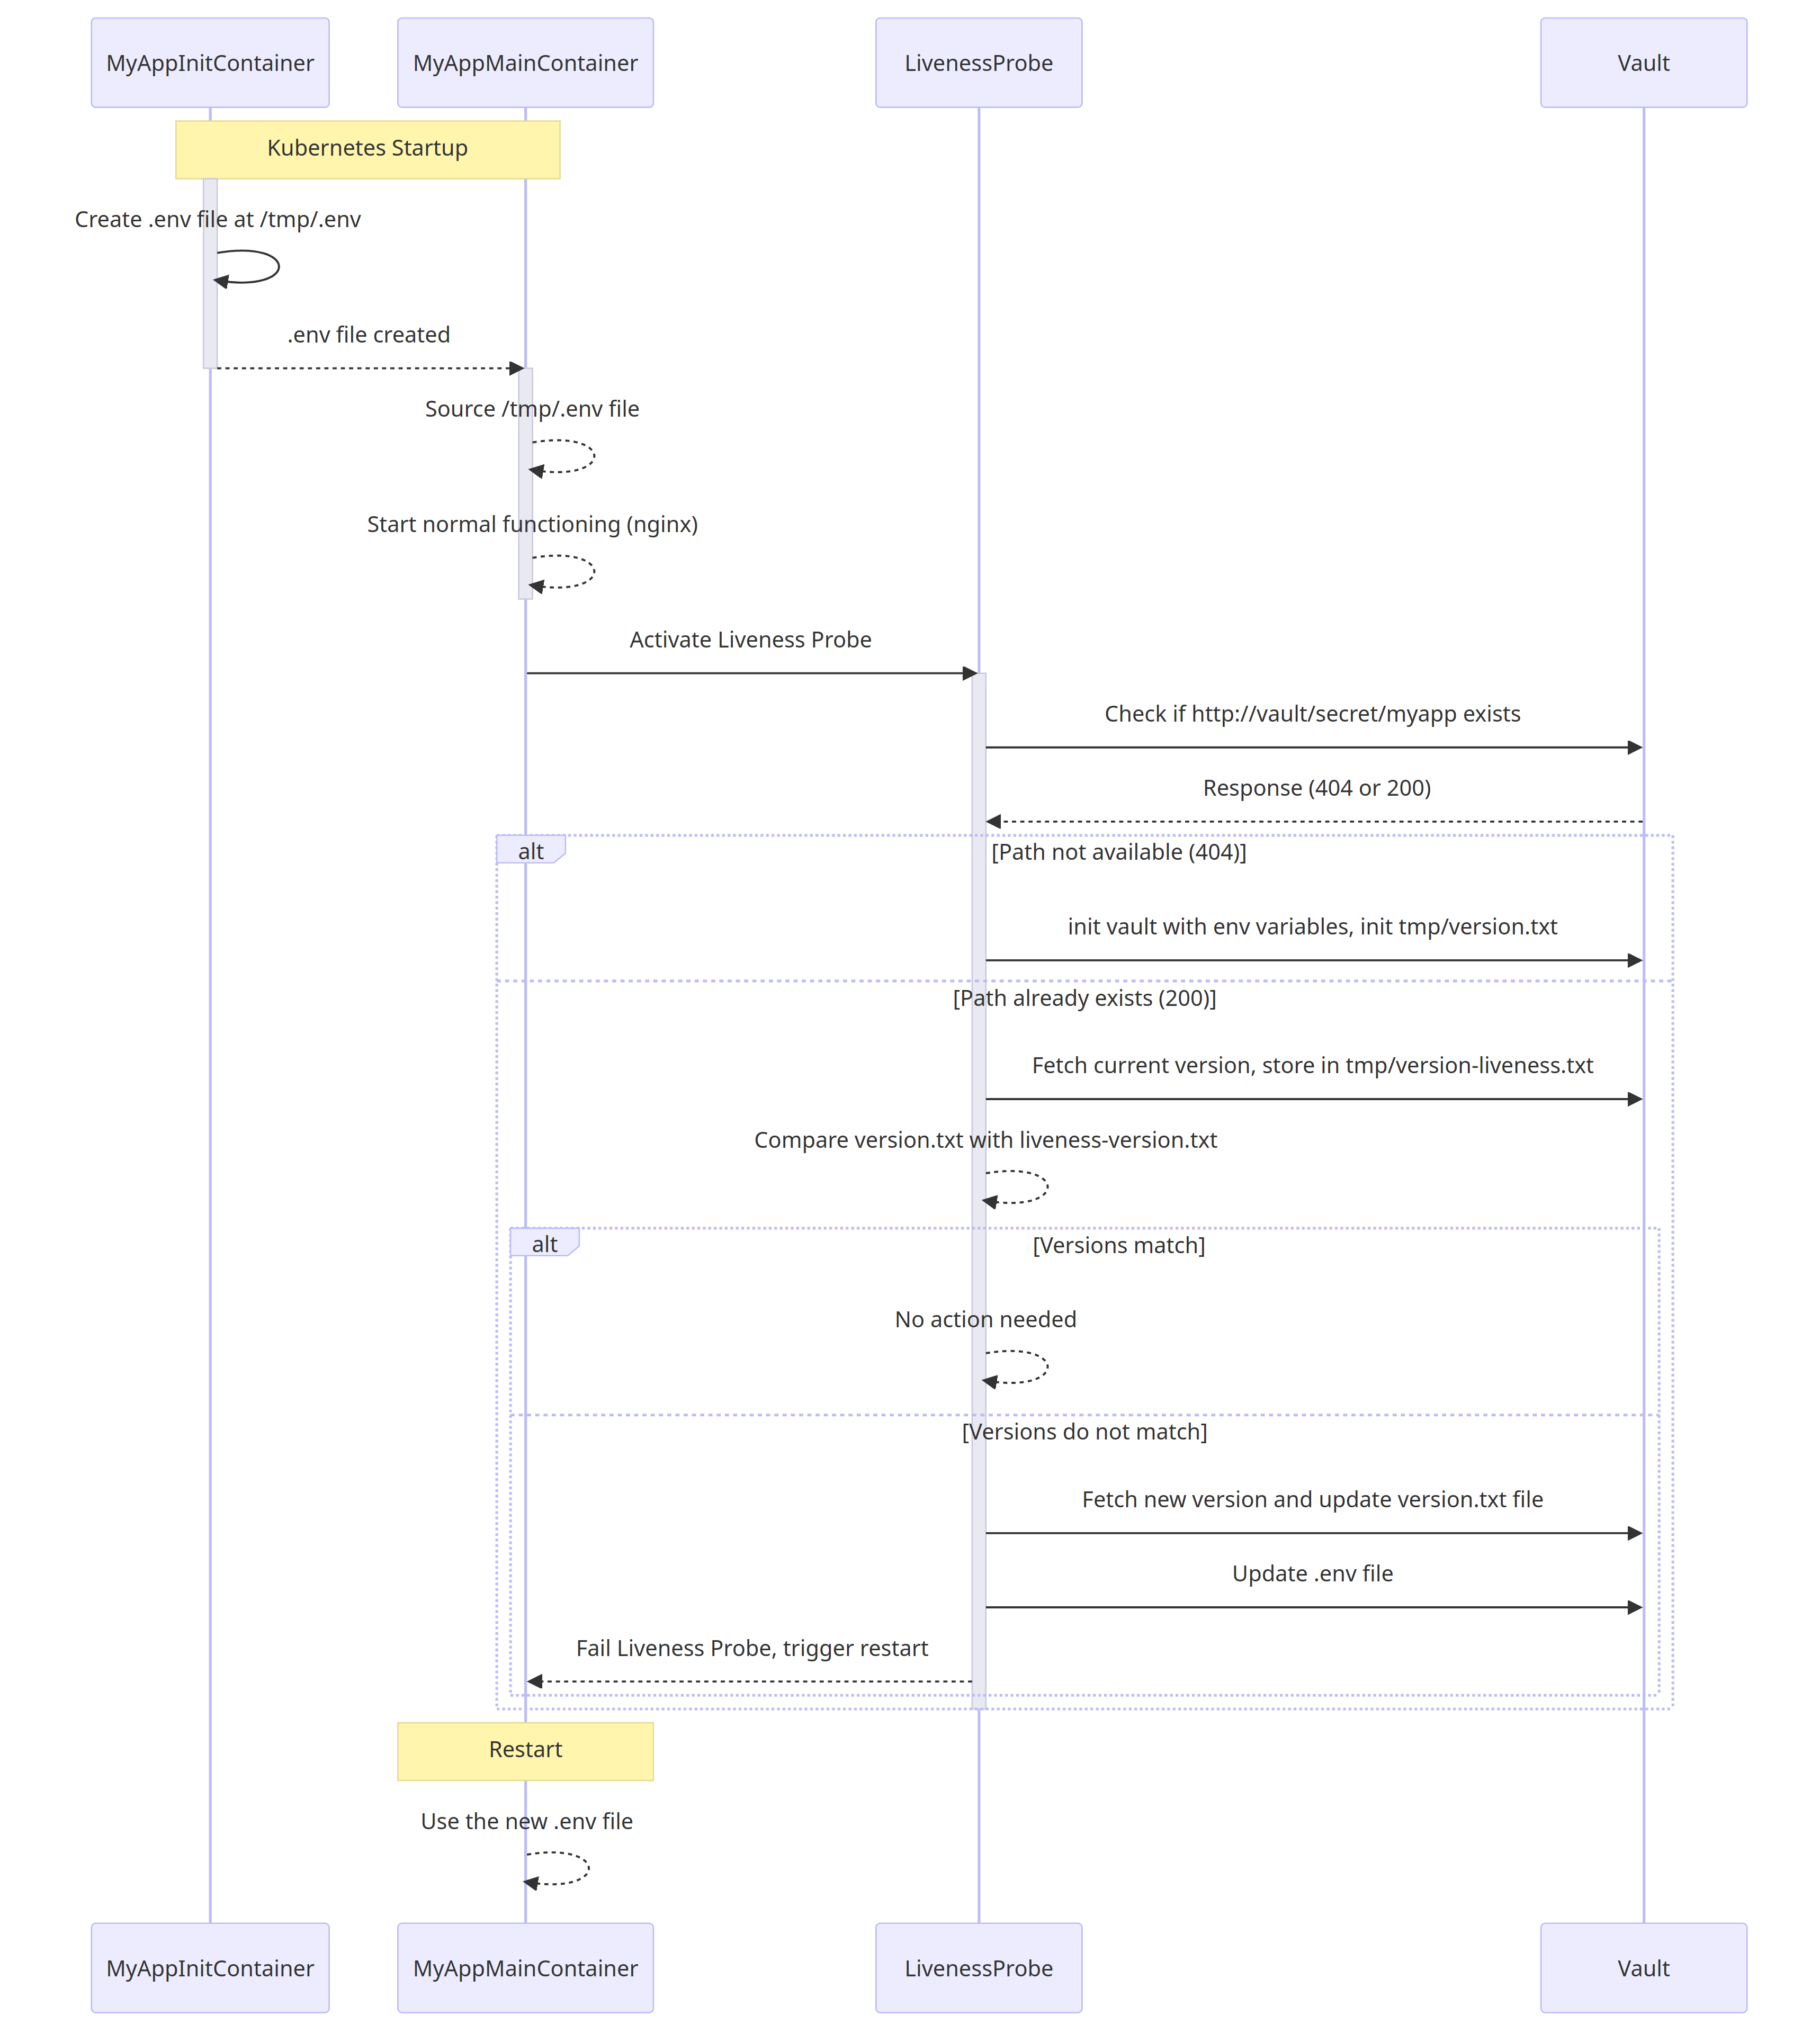
\includegraphics[width=0.8\linewidth]{figures/seq.png}
    \caption{implementation Sequence diagram}
    \label{fig:Sequence diagram}
\end{figure}


\subsection{Working}

The above diagram illustrates the sequence of events within a Kubernetes environment, depicting the initialization and operation of containers, as well as interactions with external services such as Vault for secret management. On start, Kubernetes startup triggers the activation of the \texttt{MyAppInitContainer}, responsible for generating a \texttt{.env} file at \texttt{/tmp/.env}. Subsequently, the \texttt{.env} file is passed to the \texttt{MyAppMainContainer}, which initiates normal application functionality, such as content serving via Nginx. Concurrently, the liveness probe is activated by \texttt{MyAppMainContainer}. The probe then communicates with Vault to verify the availability of a specific path (\texttt{http://vault/secret/myapp}). Depending on the response received, different paths are followed: if the path is absent (\texttt{404}), Vault initializes with environment variables and creates a version file; if present (\texttt{200}), Vault compares the current version with the locally stored version. In case of a version mismatch, Vault updates the version and \texttt{.env} files, leading to the failure of the liveness probe, triggering a restart of \texttt{MyAppMainContainer}. Upon restart, the updated \texttt{.env} file is utilized, ensuring seamless operation with the new environment. (Figure \ref{fig:Sequence diagram}).

\subsection{Kubernetes and Vault Integration}

The script provided facilitates the integration between Kubernetes and HashiCorp Vault. It begins by checking if the \texttt{VAULT\_ENABLE} environment variable is set to "true". If enabled, it proceeds to fetch secrets from Vault using the specified token and address constructed based on environment variables (\texttt{VAULT\_SERVICE\_HOST} and \texttt{VAULT\_SERVICE\_PORT}).

\subsection{Liveness Probe Implementation}

The liveness probe implementation leverages Kubernetes' built-in feature to ensure the health of containerized applications \cite{kubernetes-probes}. Within the script, an HTTP request is made to the specified Vault address to check the availability of secrets. The response status code is evaluated, and actions are taken accordingly. If the secret store is missing (404), it initializes a new Key-Vault secret path. If the token is incorrect (403), it logs an error. Otherwise, it compares the version of the retrieved secrets with the locally stored version. If a mismatch is detected, it updates the environment variables and exports them for the application to use.

\subsection{Deployment Restart Mechanism}

The deployment restart mechanism is triggered conditionally based on the outcome of the liveness probe. If the script detects changes in the environment variables fetched from Vault, it exits with a non-zero status code (1), indicating that a restart is required. This triggers Kubernetes to restart the pod, ensuring that the application picks up the updated environment variables. Conversely, if no changes are detected, the script exits with a zero status code (0), indicating that the environment variables are up to date, and no restart is necessary. This mechanism ensures that the application remains consistent to configuration changes and always uses the latest variables from Vault.

\section{Integration}

To start, the code implementation can be accessed at \url{https://github.com/pranay-bh/helm-keycloak} for basic deployment guideline.
To integrate HashiCorp Vault into a generic deployment, follow the outlined procedure:

\begin{enumerate}
  \item \textbf{Deploy HashiCorp Vault:} Begin by deploying HashiCorp Vault within your environment. This provides a UI to change environment variables.
  
  \item \textbf{Configure Config Map:} Create a config map containing a shell script named \texttt{vault-integration.sh} from the GitHub repository mentioned architecture. 
  \begin{itemize}
    \item  This script takes two parameters:
    \begin{itemize}
      \item \textbf{Vault Token:} By default, set to 'admin'.
      \item \textbf{Vault Path:} This path acts as the location in Vault where the variables will be stored. Adjust this path if needed.
    \end{itemize}
    If Vault is running in a different cluster: Update the Vault Path to reach the URL and Vault token of the external Vault instance.
  \end{itemize}
  
  \item \textbf{Values.yaml File:} Ensure that the \texttt{values.yaml} file includes the following variables \newline
      Vault\_Token
      Vault\_Path
      Vault\_Enabled
  
  \item \textbf{Update Deployment Container:}
  \begin{itemize}
    \item Add two volume mounts:
    \begin{itemize}
      \item For bash scripts (config and secret YAML file mounts are read-only after Kubernetes 1.19) (in previous script:, \texttt{/var/tmp}).
      \item For writing the \texttt{.env} file and temporary files to compare Vault secret versions (in previous script:, \texttt{/tmp}).
    \end{itemize}
    \item Create an init container responsible for creating a new \texttt{.env} file. This file stores all variables required for the main container's startup. Its absence may cause the main container to fail to start.
    \item Mount volumes and pass Vault-specific environment variables to the main container.
    \item Create and execute a script from the liveness probe to interact with Vault.
  \end{itemize}
\end{enumerate}

\section{Risks}
The above mentioned deployment structure posses some potential risks. Firstly, Vault serves as the single source of failure within the system. Any downtime or service interruption of the Vault instance could disrupt critical operations reliant on its services. 

Moreover, without proper backup mechanisms, such as persistent storage or integration with Consul for Vault, the loss of Vault data upon restart poses a significant risk. To mitigate this, implementing persistence storage with Vault or utilizing Consul for Vault management can enhance data reliability and availability. 

Additionally, containerized applications must be configured to correctly source environment variables from the Vault setup. Misconfiguration can lead to applications failing to accessing updated environment variables.

Thus, while Vault integration offers numerous benefits, careful consideration and implementation of mitigating measures are essential to address these potential risks effectively.
\section{Result}

The result addresses the challenges posed by manual configuration in Kubernetes deployments, offering a robust, UI Based automated solution to intelligently inject environment variables into Kubernetes clusters. The solution not only eliminates the need for manual tweaking and adjustment but also make developers to do the same task without having knowledge of deployments and infrastructure. It enhances reliabilit and scalability within dynamic environments where configuration changes are frequent.
The solution includes a script packaged along with the application container image or as a ConfigMap in Kubernetes, ensuring availability within the container environment and execution as part of the pod lifecycle.

During pod initialization, Kubernetes mounts the script and executes it as a liveness probe. The script communicates with HashiCorp Vault using the specified address and token to fetch secrets as needed. Standard Unix commands such as \texttt{curl} and \texttt{jq} are utilized to interact with the Vault API and parse JSON responses. Upon detecting changes in retrieved secrets, the script restart the pods and exports new secrets as environment variables within the pod, ensuring the application has access to the latest configuration.

The result addresses the problem statement by providing an automated solution that intelligently manages environment variables, enhancing the reliability, security, and scalability of applications running in Kubernetes clusters. By automatically triggering pod restarts upon detecting changes or updates to the configuration, the solution minimizes errors, inconsistencies, and downtime, thereby optimizing the operational efficiency of Kubernetes deployments.
\section{Conclusion}
\lipsum[2]

\subsection{Citation example}
Hawthorn et al. \cite{Reference1} talk about laser, which is similar to the work of his colleagues \cite{Reference2, Reference3}.

\subsection{Table and listing example}
\Cref{tab:treatments} shows an example for a table in \LaTeX.

\begin{table}[th]
\caption{The effects of treatments X and Y on the four groups studied.}
\label{tab:treatments}
\centering
\begin{NiceTabular}{lrr}
\CodeBefore
\rowcolors{2}{gray!10}{white}
\Body
\textbf{Groups} & \textbf{Treatment X} & \textbf{Treatment Y} \\
1 & 0.20 & 0.80\\
2 & 0.17 & 0.70\\
3 & 0.24 & 0.75\\
4 & 0.68 & 0.30\\
\end{NiceTabular}
\end{table}

[If you show results in tables, always ensure all of them are aligned to the right and have the same precision.]

\Cref{lst:hello} shows an example of a listing, a good way to display code in \LaTeX.

\begin{listing}[th]
	\begin{minted}{Go}
package main
import "fmt"
func main() {
    fmt.Println("Hello, world!")
}
	\end{minted}
\caption{"Hello, world!" in Go}
\label{lst:hello}
\end{listing}





\newpage
\printbibliography{}
\newpage

% --- your appendix ---
\appendix
\break

\pagenumbering{arabic}
\renewcommand*{\thepage}{A\arabic{page}}

\section{Code samples}

% Define settings for code listings
\lstset{
    basicstyle=\small\ttfamily,
    breaklines=true,
    postbreak=\mbox{\textcolor{red}{$\hookrightarrow$}\space},
    numbers=left,
    numberstyle=\tiny,
    stepnumber=1,
    showstringspaces=false,
    tabsize=2,
    captionpos=b,
    frame=single
}


\begin{lstlisting}[language=bash, caption={liveness probe bash script}, label={lst:your_script}]
if [ "$VAULT_ENABLE" = "true" ]; then

    VAULT_TOKEN="admin"
    VAULT_PATH="myapp"
    VAULT_ADDRESS="http://$VAULT_SERVICE_HOST:$VAULT_SERVICE_PORT/v1/secret/data/$VAULT_PATH"
    echo "address: " $VAULT_ADDRESS
    VAULT_HEADER="X-Vault-Token: $VAULT_TOKEN"

    echo "Installing necessary packages: curl and jq..."
    which apt-get && apt-get update && apt-get install -y curl jq
    curl
    jq

    HTTP_STATUS_CODE=$(curl -s --location "$VAULT_ADDRESS" --header "X-Vault-Token: $VAULT_TOKEN" -o /dev/null -w "%{http_code}")

    if [ "$HTTP_STATUS_CODE" = "000" ]; then
        echo "Service not found on given URL: $VAULT_ADDRESS"
        exit 0
    elif [ "$HTTP_STATUS_CODE" = "404" ]; then
        echo "Store does not exist. Initializing Vault store in $VAULT_PATH for the first time..."
        BODY=$(env | sort | jq -R -n 'reduce inputs as $line ({}; . + ($line | split("=") | {(.[0]): .[1]})) | {"data": .}')
        curl -s -H "$VAULT_HEADER" -H "Content-Type: application/json" -X POST -d "$BODY" "$VAULT_ADDRESS" -o /dev/null
        echo 1 > /tmp/version.txt
        exit 0
    elif [ "$HTTP_STATUS_CODE" = "403" ]; then
        echo "Incorrect token: $VAULT_TOKEN for $VAULT_ADDRESS"
        exit 0
    else
        echo "Status code: $HTTP_STATUS_CODE"
        echo "$(curl -s -H "$VAULT_HEADER" "$VAULT_ADDRESS" | jq -r '.data.metadata.version')" > /tmp/liveness-version.txt

        if cmp -s /tmp/version.txt /tmp/liveness-version.txt; then 
            echo "Environment variable version $(cat /tmp/liveness-version.txt) is up to date"
            exit 0
        else
            echo "New environment variable version $(cat /tmp/liveness-version.txt) detected"
            JSON_DATA="$(curl -s -H "$VAULT_HEADER" "$VAULT_ADDRESS")"
            echo "$( echo $JSON_DATA | jq -r '.data.metadata.version')" > /tmp/version.txt
            rm /tmp/.env || true
            echo "Exporting variables for $VAULT_PATH with version $(cat /tmp/version.txt)"
            keys=$(echo "$JSON_DATA" | jq -r '.data.data | keys[]')
            for key in $keys; do
                value=$(echo "$JSON_DATA" | jq -r ".data.data[\"$key\"]")
                export "$key"="$value"
                # echo "Exporting variable: $key=$value"
                echo "$key=\"$value\"" >> /tmp/.env
            done
            exit 1
        fi
    fi
else
    echo "VAULT_ENABLE is not set to true. Doing nothing and moving on as expected."
fi
\end{lstlisting}

\end{document}
 